%%%%%%%%%%%%%%%%%%%%%%%%%%%%%%%%%%%%%%%%%
% Jacobs Landscape Poster
% LaTeX Template
% Version 1.1 (14/06/14)
%
% Created by:
% Computational Physics and Biophysics Group, Jacobs University
% https://teamwork.jacobs-university.de:8443/confluence/display/CoPandBiG/LaTeX+Poster
% 
% Further modified by:
% Nathaniel Johnston (nathaniel@njohnston.ca)
%
% This template has been downloaded from:
% http://www.LaTeXTemplates.com
%
% License:
% CC BY-NC-SA 3.0 (http://creativecommons.org/licenses/by-nc-sa/3.0/)
%
%%%%%%%%%%%%%%%%%%%%%%%%%%%%%%%%%%%%%%%%%

%----------------------------------------------------------------------------------------
%	PACKAGES AND OTHER DOCUMENT CONFIGURATIONS
%----------------------------------------------------------------------------------------

\documentclass[final]{beamer}

\usepackage[scale=1.24]{beamerposter} % Use the beamerposter package for laying out the poster

\usetheme{confposter} % Use the confposter theme supplied with this template

\usepackage[english]{babel}
\usepackage[utf8x]{inputenc}
\usepackage{physics}
\usepackage{graphicx, caption}
\usepackage{tcolorbox}
\usepackage{amsmath}
\usepackage[mathscr]{euscript}
\usepackage[absolute,overlay]{textpos}
%\usepackage{algorithmicx}
%\usepackage[Algorithm,ruled]{algorithm}
\usepackage{tikz}
\usetikzlibrary{tikzmark}
\usepackage{calc}
\usepackage{times}
\usepackage{tikz}
\usetikzlibrary{shapes.geometric, arrows}
\usepackage{colortbl}


\setbeamercolor{block title}{fg=ngreen,bg=white} % Colors of the block titles
\setbeamercolor{block body}{fg=black,bg=white} % Colors of the body of blocks
\setbeamercolor{block alerted title}{fg=white,bg=dblue!70} % Colors of the highlighted block titles
\setbeamercolor{block alerted body}{fg=black,bg=dblue!10} % Colors of the body of highlighted blocks
% Many more colors are available for use in beamerthemeconfposter.sty

%-----------------------------------------------------------
% Define the column widths and overall poster size
% To set effective sepwid, onecolwid and twocolwid values, first choose how many columns you want and how much separation you want between columns
% In this template, the separation width chosen is 0.024 of the paper width and a 4-column layout
% onecolwid should therefore be (1-(# of columns+1)*sepwid)/# of columns e.g. (1-(4+1)*0.024)/4 = 0.22
% Set twocolwid to be (2*onecolwid)+sepwid = 0.464
% Set threecolwid to be (3*onecolwid)+2*sepwid = 0.708

\newlength{\sepwid}
\newlength{\onecolwid}
\newlength{\twocolwid}
\newlength{\threecolwid}
\setlength{\paperwidth}{48in} % A0 width: 46.8in
\setlength{\paperheight}{36in} % A0 height: 33.1in
\setlength{\sepwid}{0.024\paperwidth} % Separation width (white space) between columns
\setlength{\onecolwid}{0.22\paperwidth} % Width of one column
\setlength{\twocolwid}{0.464\paperwidth} % Width of two columns
\setlength{\threecolwid}{0.708\paperwidth} % Width of three columns
\setlength{\topmargin}{-0.5in} % Reduce the top margin size
%-----------------------------------------------------------

\usepackage{graphicx}  % Required for including images

\usepackage{booktabs} % Top and bottom rules for tables

%----------------------------------------------------------------------------------------
%	TITLE SECTION 
%----------------------------------------------------------------------------------------


%\title{High-Dimensional Semi-Quantum Cryptography} % Poster title

\title{%
	\texorpdfstring{%
		\makebox[\linewidth]{%
			\makebox[0pt][l]{%
				\raisebox{\dimexpr-\height+\baselineskip}[0pt][0pt]
				{
\includegraphics[height=2.5\baselineskip]{leaf.jpg}}% Left logo
			}\hfill
			\makebox[0pt]{High-Dimensional Semi-Quantum Cryptography}%
			\hfill\makebox[0pt][r]{%
				\raisebox{\dimexpr-\height+\baselineskip}[0pt][0pt]
				{
\includegraphics[height=2.5\baselineskip]{leaf.jpg}}% Right logo
			}%
		}%
	}
	{High-Dimensional Semi-Quantum Cryptography}} % Poster title

\author{Hasan Iqbal, Walter O. Krawec} % Author(s)

\institute{Computer Science and Engineering, UConn} % Institution(s)

%----------------------------------------------------------------------------------------

\begin{document}

%
\includegraphics[]{uconn.png}
%
\includegraphics[]{husky.jpg}

\addtobeamertemplate{block end}{}{\vspace*{2ex}} % White space under blocks
\addtobeamertemplate{block alerted end}{}{\vspace*{2ex}} % White space under highlighted (alert) blocks

\setlength{\belowcaptionskip}{2ex} % White space under figures
\setlength\belowdisplayshortskip{2ex} % White space under equations

\begin{frame}[t] % The whole poster is enclosed in one beamer frame

\begin{columns}[t] % The whole poster consists of three major columns, the second of which is split into two columns twice - the [t] option aligns each column's content to the top

\begin{column}{\sepwid}\end{column} % Empty spacer column

\begin{column}{\onecolwid} % The first column

%----------------------------------------------------------------------------------------
%	OBJECTIVES
%----------------------------------------------------------------------------------------

\begin{alertblock}{Objectives}
\textbf{Can we have unconditional communication security with limited quantum resources?}
\begin{itemize}
%\item Restrict one parties capability. 
\item Bridge the gap between classical and quantum realm.
\item Use less expensive quantum hardwares.
\item Fallback option for fully-fledged quantum key distribution.
\end{itemize}

\end{alertblock}

%----------------------------------------------------------------------------------------
%	INTRODUCTION
%----------------------------------------------------------------------------------------

\begin{block}{Motivation}

\begin{itemize}
\item Unconditional security is impossible with all-classical capabilities but possible with quantum resources. 
\item High-dimensional QKD offers better protection.
\item Using HD-resources in SQKD provides advantages. 
\end{itemize}

\end{block}


\begin{block}{What is Quantum Key Distribution}
	
	\begin{figure}
		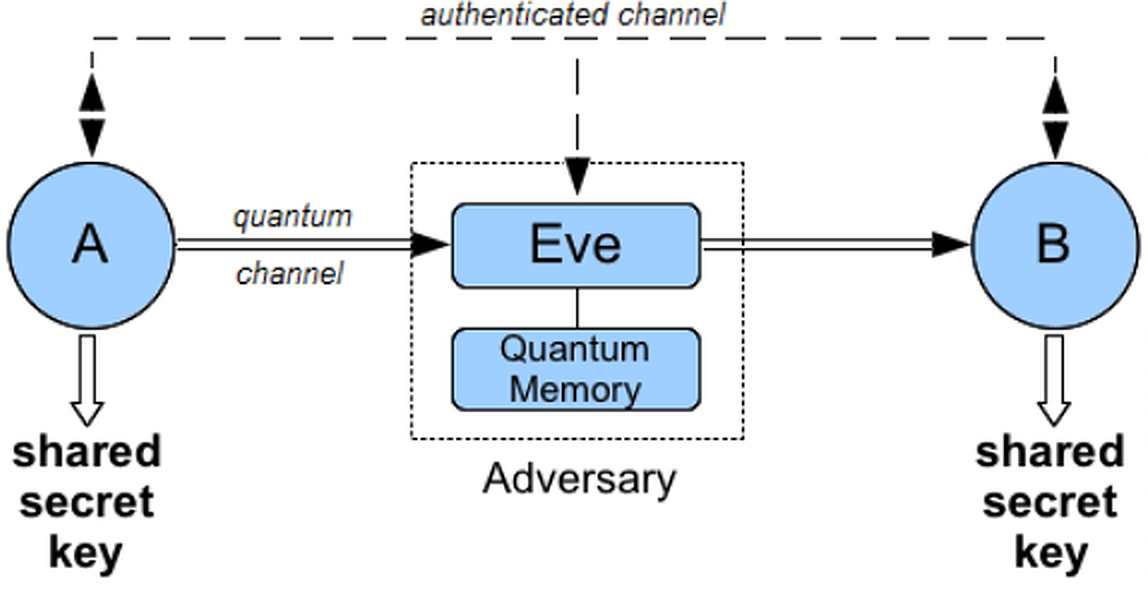
\includegraphics[width=\linewidth]{qkd.png}
		\caption{Quantum Key Distribution}
	\end{figure}
\begin{itemize}
\item Alice sends her friend Bob information via qubit through quantum channel.
\item Adversary Eve can attack the channel in various ways.
\item Alice and Bob communicates classically to produce a shared key.
\item The key is secure as long as Eve does not know 'too much' about it compared to Bob.
\end{itemize}	
	
\end{block}

%----------------------------------------------------------------------------------------

\end{column} % End of the first column


\begin{column}{\sepwid}\end{column} % Empty spacer column

\begin{column}{\twocolwid} % Begin a column which is two columns wide (column 2)

\begin{columns}[t,totalwidth=\twocolwid] % Split up the two columns wide column

\begin{column}{\onecolwid}\vspace{-.6in} % The first column within column 2 (column 2.1)

%----------------------------------------------------------------------------------------
%	MATERIALS
%----------------------------------------------------------------------------------------

\begin{block}{What is High-Dimensional SQKD}

\begin{itemize}
\item High-Dimensional qudits instead of traditional qubits. 
\item More information transmitted in each iteration. 
\item Robust against quantum cloning.
\item Better noise resistance. 
\end{itemize}

\begin{figure}
	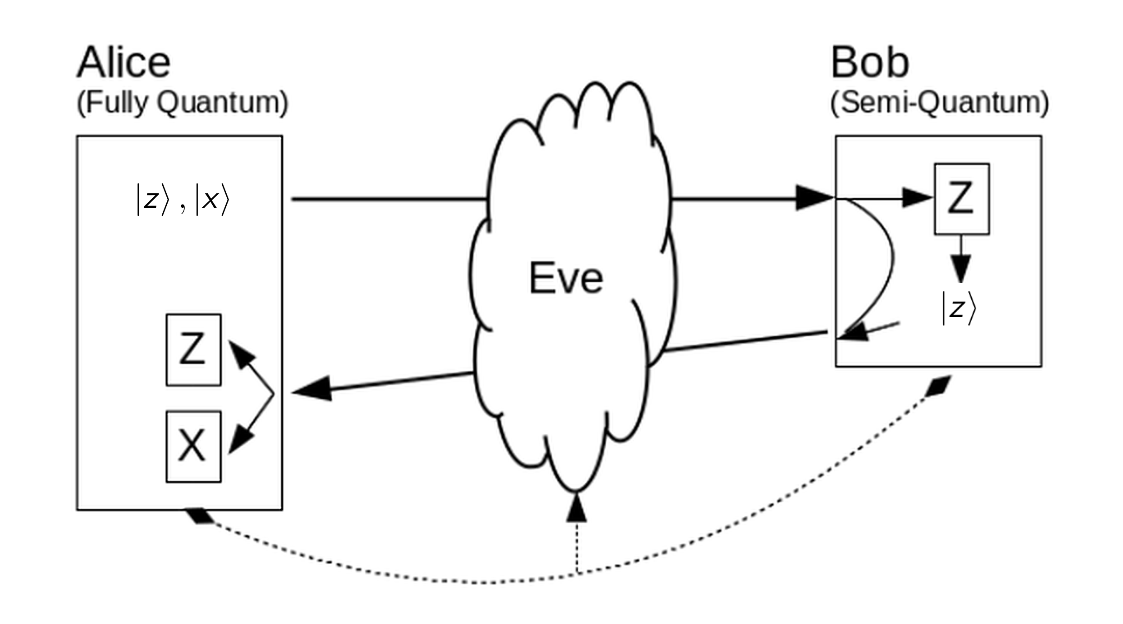
\includegraphics[width=\linewidth]{sqkd_hidim}
	\caption{High-dimensional SQKD}
	\label{fig:sqkd_hidim}
\end{figure}


\end{block}

%----------------------------------------------------------------------------------------

\end{column} % End of column 2.1

\begin{column}{\onecolwid}\vspace{-.6in} % The second column within column 2 (column 2.2)

%----------------------------------------------------------------------------------------
%	METHODS
%----------------------------------------------------------------------------------------

\begin{block}{Reduction Process}
\begin{figure}
	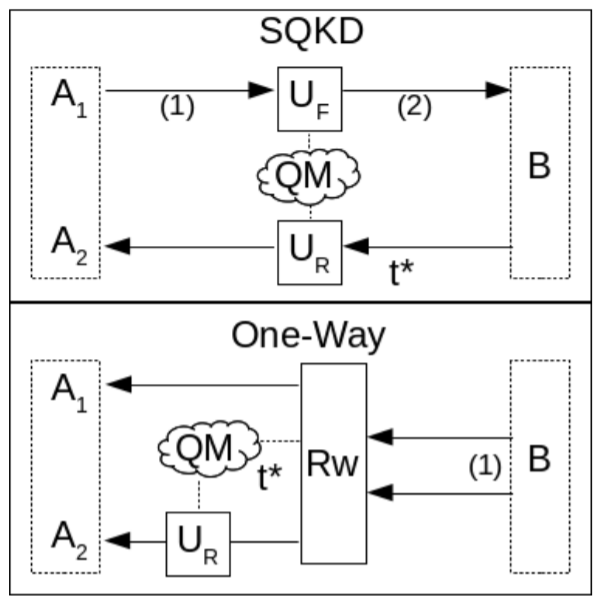
\includegraphics[width=0.8\linewidth]{oneway.png}
	\caption{Convert two-way attack to one-way using a special attack operator $R_w$ }
\end{figure}


\end{block}

%----------------------------------------------------------------------------------------

\end{column} % End of column 2.2

\end{columns} % End of the split of column 2 - any content after this will now take up 2 columns width

%----------------------------------------------------------------------------------------
%	IMPORTANT RESULT
%----------------------------------------------------------------------------------------

\begin{alertblock}{Important Result}
High-dimensional SQKD offers the best key-rate so far. Proof simplification technique developed here is applicable to other quantum key distribution protocols.
\end{alertblock} 

%----------------------------------------------------------------------------------------

\begin{columns}[t,totalwidth=\twocolwid] % Split up the two columns wide column again

\begin{column}{\onecolwid} % The first column within column 2 (column 2.1)

%----------------------------------------------------------------------------------------
%	MATHEMATICAL SECTION
%----------------------------------------------------------------------------------------

\begin{block}{Simplified Protocol}

%\begin{figure}
%	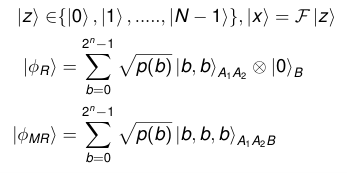
\includegraphics[width=.6\linewidth]{hd_eqns.png}
%\end{figure}

%\begin{itemize}
%\item We propose HD-SQKD to achieve the objectives. 
%\item To reduce analysis complexity of HD-SQKD, we show another equivalent protocol OW-SQKD. 
%\end{itemize}

      \begin{tabular}{|p{14cm}|p{14cm}|}
      	\hline 
      	\textbf{HD-SQKD} & \textbf{OW-SQKD}\\
      	\hline \hline
      	1. Alice prepares $\ket{z}$ or $\ket{x}$, sends to Bob.  & 1. Bob prepares and sends two different states based on measure-resend or reflect.\\ \hline
      	2. Eve attacks the forward channel.  & 2. Eve attacks only once. \\ \hline
      	3. Bob measure-resends or reflects. & 3. Alice measures in two basis. \\ \hline
      	4. Eve attacks the reverse channel. &  \\ \cline{1-1}      	
		5. Alice measures the returning qubits.  & \\ \hline
      \end{tabular}

%\begin{figure}
%	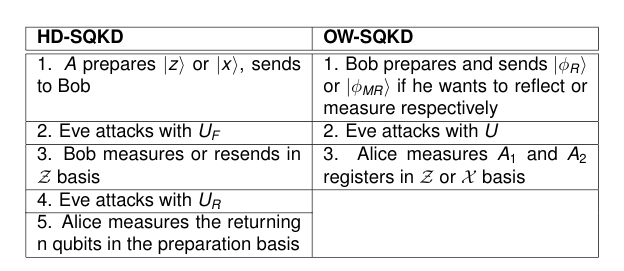
\includegraphics[width=1.09\linewidth]{hd_v_ow.png}
%\end{figure}


\end{block}

%----------------------------------------------------------------------------------------

\end{column} % End of column 2.1

\begin{column}{\onecolwid} % The second column within column 2 (column 2.2)

%----------------------------------------------------------------------------------------
%	RESULTS
%----------------------------------------------------------------------------------------

\begin{block}{Evaluation}

\begin{itemize}
\item Noise tolerance: How much disturbance in the channel can the protocol withstand. 
\item How does it compare to a famous fully quantum HD-QKD protocol.
\end{itemize}
\begin{figure}
	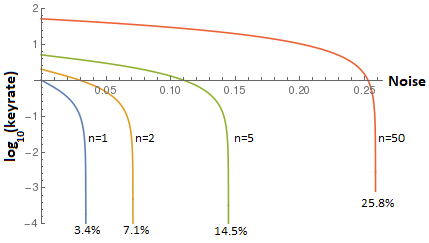
\includegraphics[width=.9\linewidth]{keyrate-ind.png}
	\caption{Noise Tolerance in different dimensions}
	\end{figure}

%\begin{figure}
%	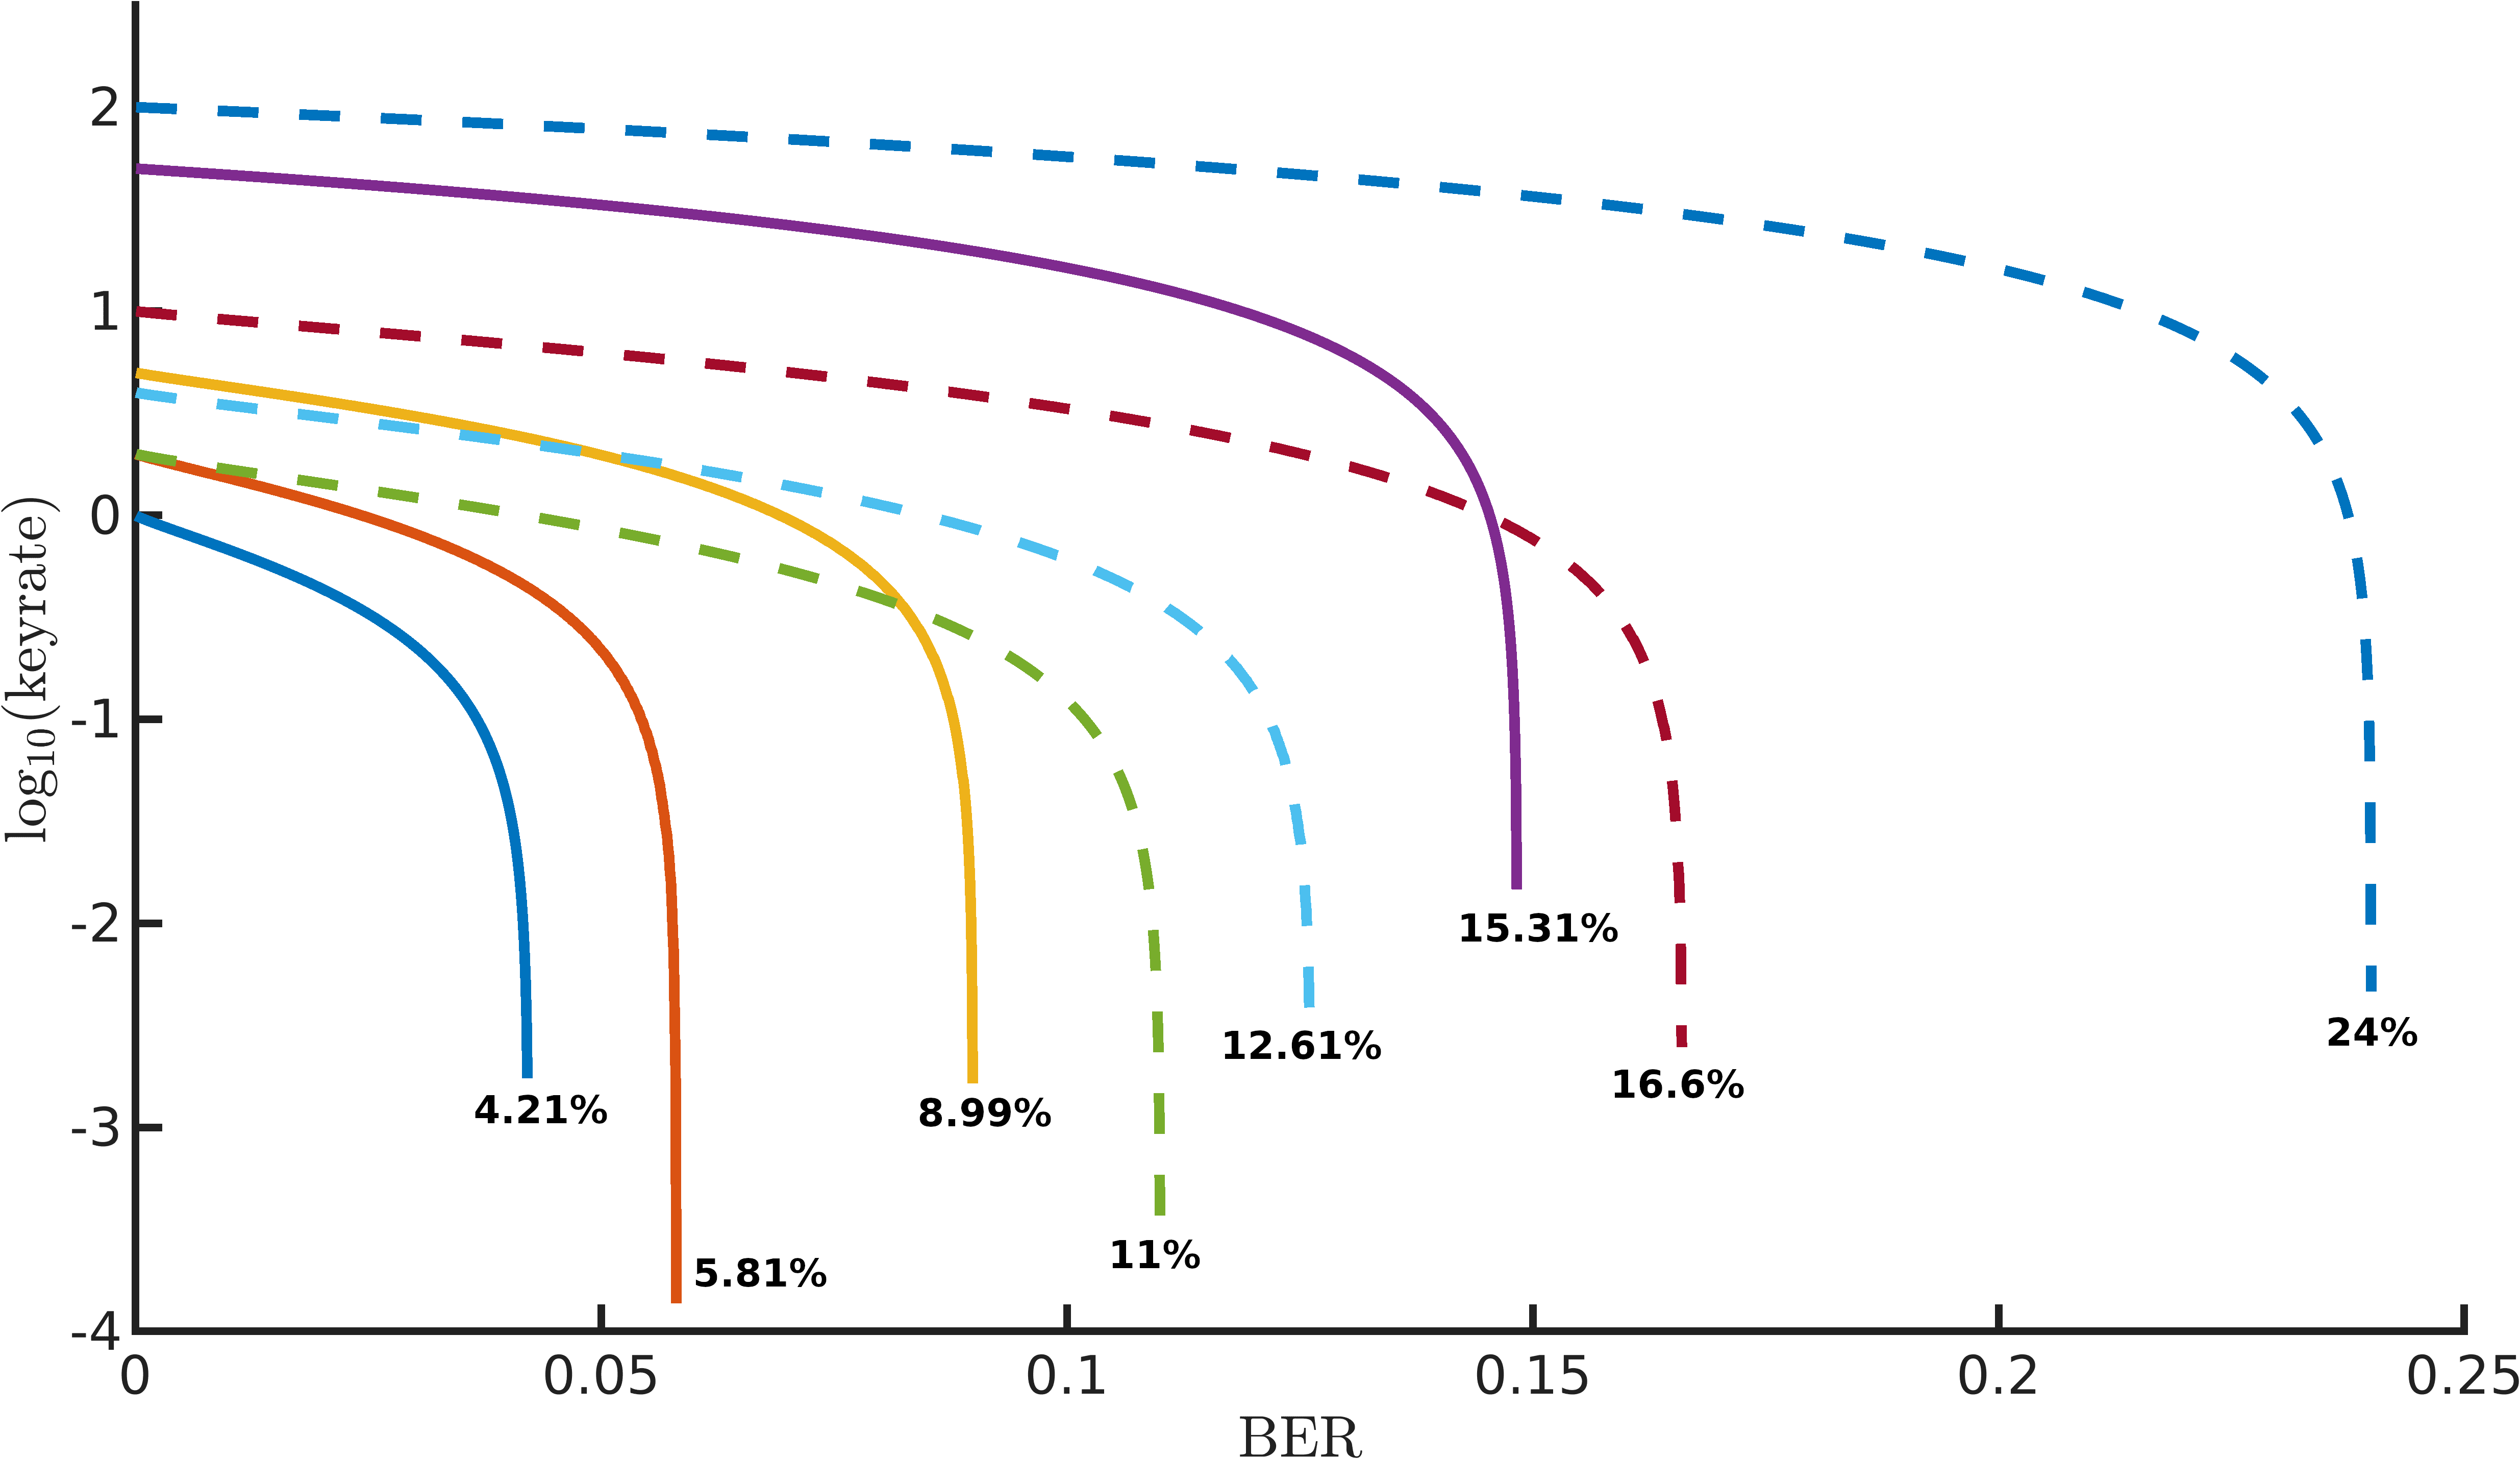
\includegraphics[width=\linewidth]{ber_v_kr_to_label_done_small.png}
%	\caption{Bit error rate vs Key rate: HD-SQKD vs HD-BB84}
%\end{figure}



\end{block}

%----------------------------------------------------------------------------------------

\end{column} % End of column 2.2

\end{columns} % End of the split of column 2

\end{column} % End of the second column

\begin{column}{\sepwid}\end{column} % Empty spacer column

\begin{column}{\onecolwid} % The third column

%----------------------------------------------------------------------------------------
%	CONCLUSION
%----------------------------------------------------------------------------------------

\begin{figure}
	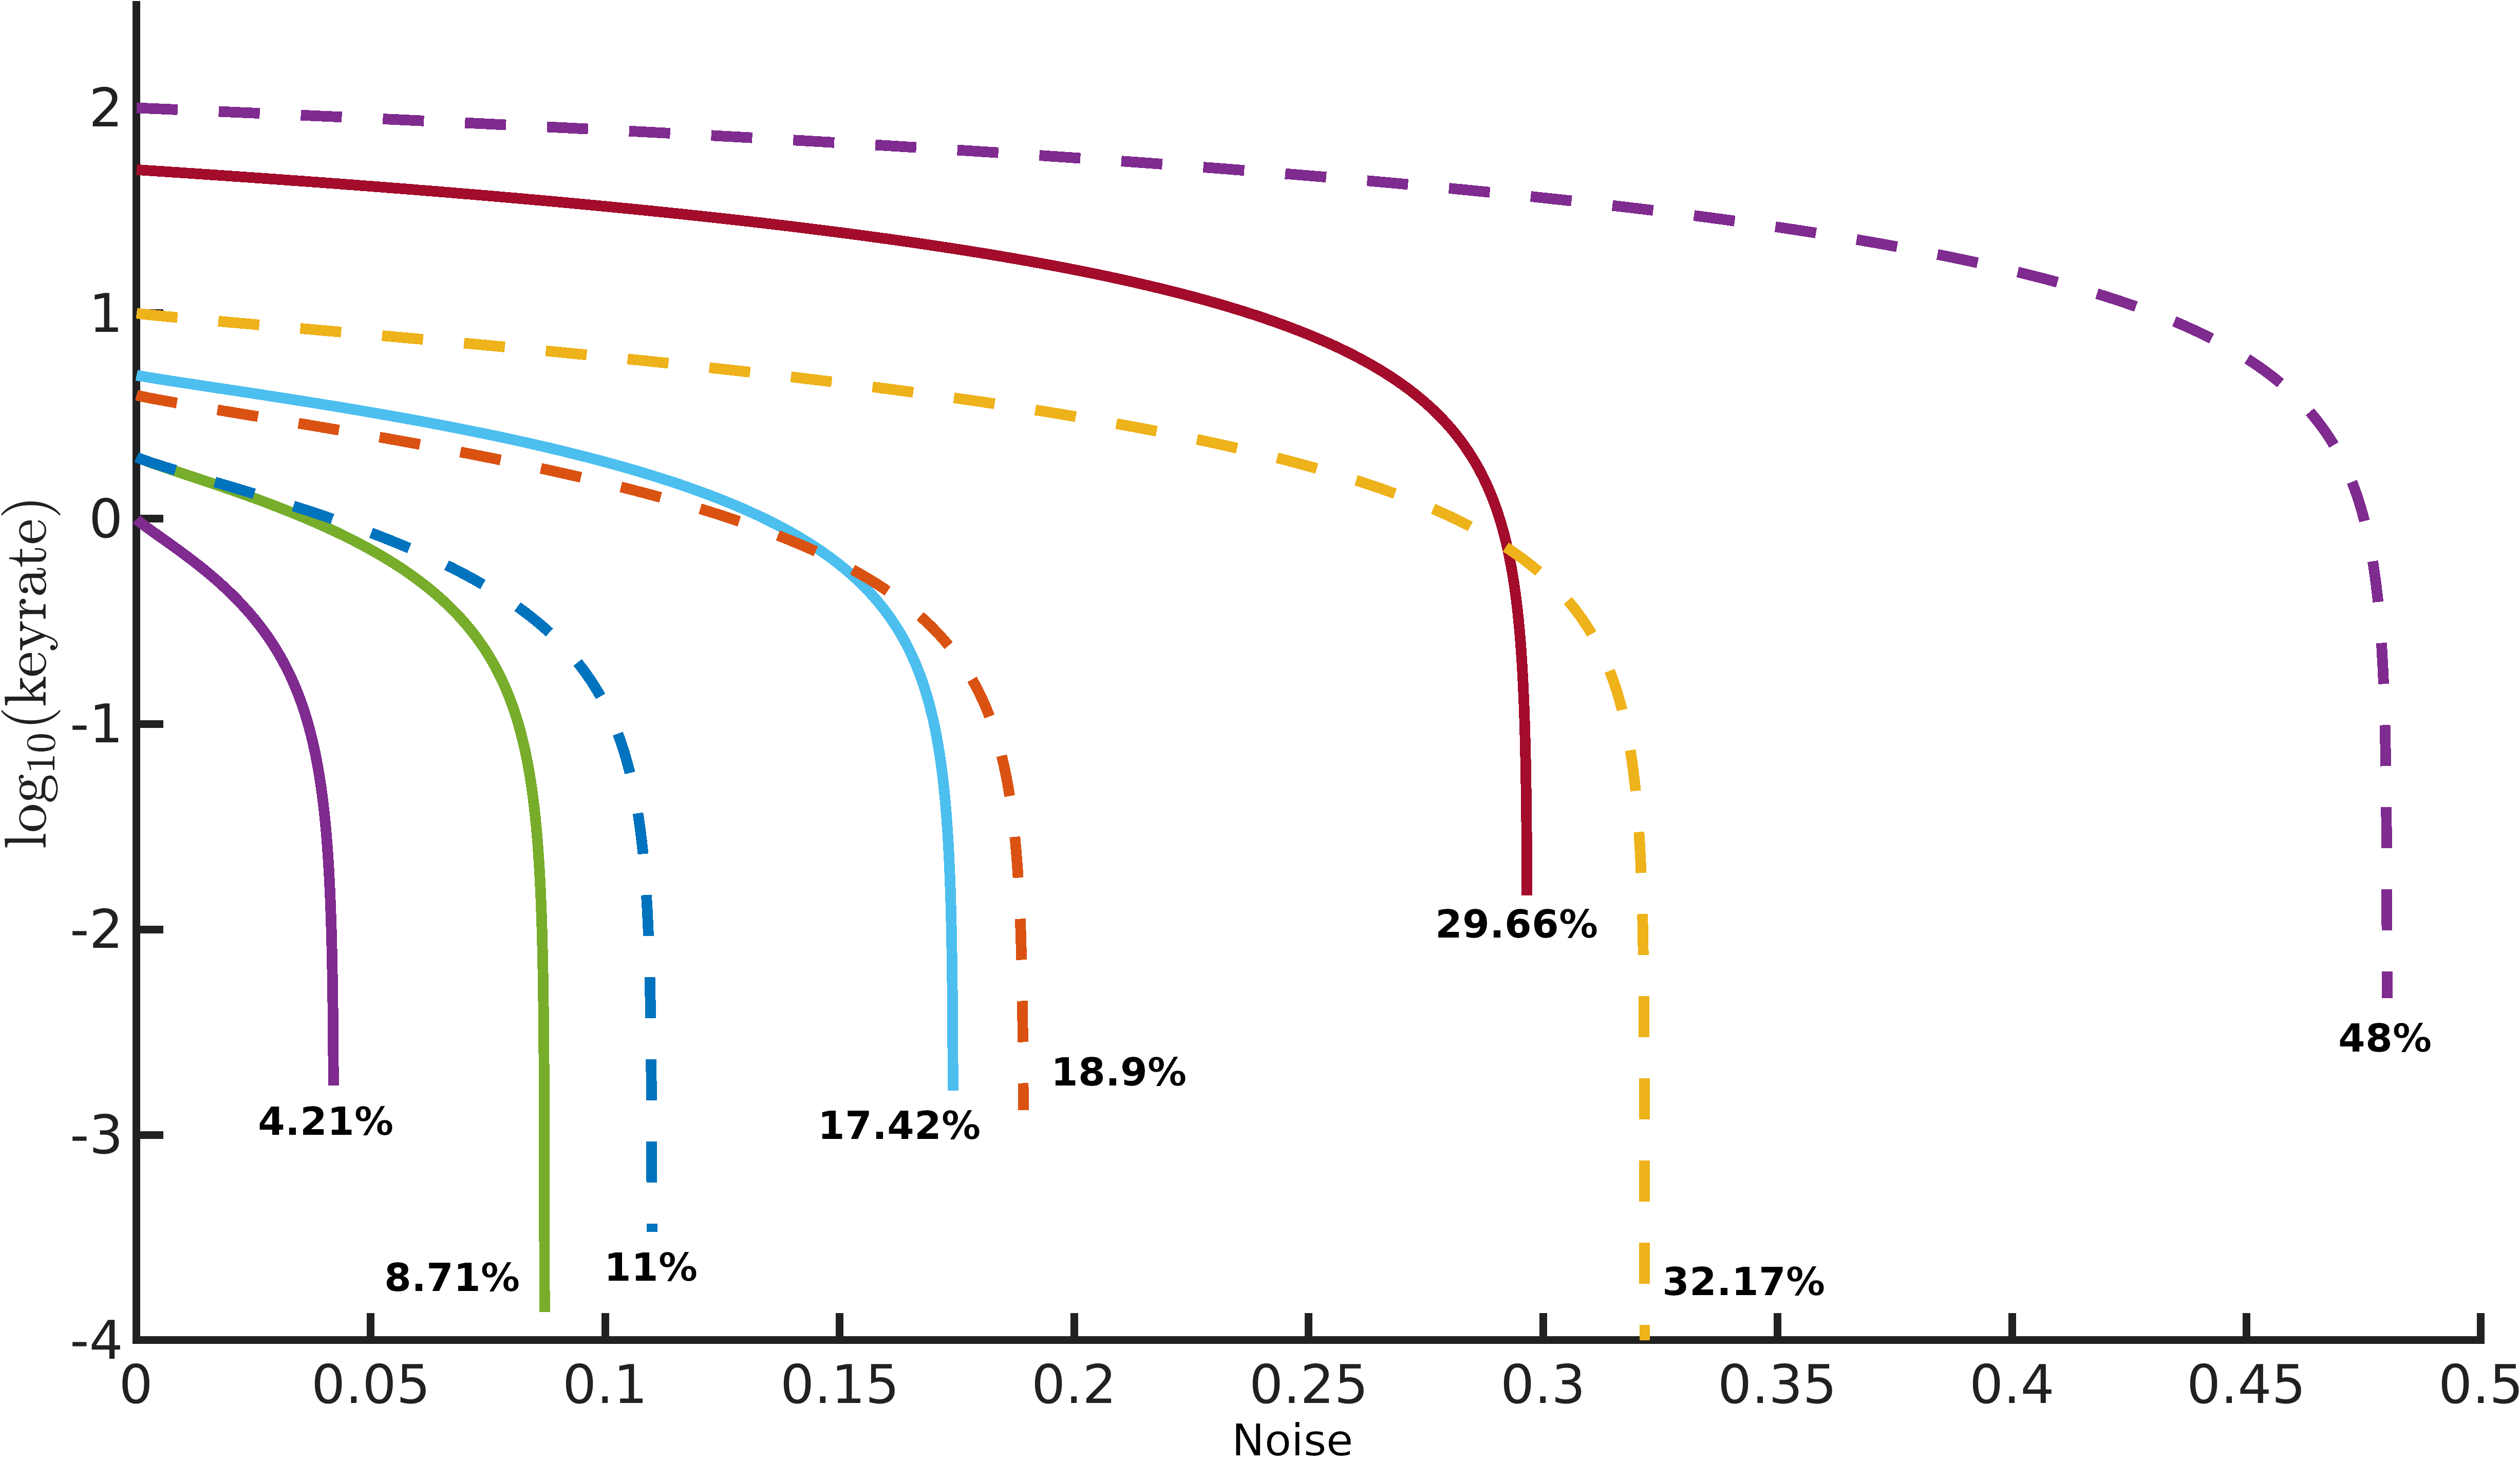
\includegraphics[width=\linewidth]{q_v_kr_to_label_done_small.png}
	\caption{Noise vs Key rate: HD-SQKD vs HD-BB84}
\end{figure}

\begin{block}{Conclusion}

\begin{itemize}
	\item We have proposed a new HD-SQKD protocol.
	\item Performed an information-theoretic security analysis. 
	\item Showed how to reduce a two-way protocol to one way. 
	\item Proved that qudits can indeed benefit SQKD model. 
	\item Applying this proof technique to other protocols would be quite interesting. 
\end{itemize}

\end{block}

%----------------------------------------------------------------------------------------
%	ADDITIONAL INFORMATION
%----------------------------------------------------------------------------------------
%
%\begin{block}{Additional Information}
%
%Maecenas ultricies feugiat velit non mattis. Fusce tempus arcu id ligula varius dictum. 
%\begin{itemize}
%\item Curabitur pellentesque dignissim
%\item Eu facilisis est tempus quis
%\item Duis porta consequat lorem
%\end{itemize}
%
%\end{block}

%----------------------------------------------------------------------------------------
%	REFERENCES
%----------------------------------------------------------------------------------------

\begin{block}{References}

\nocite{*} % Insert publications even if they are not cited in the poster
\small{\bibliographystyle{unsrt}
\bibliography{sample}\vspace{0.75in}}

\end{block}

%----------------------------------------------------------------------------------------
%	ACKNOWLEDGEMENTS
%----------------------------------------------------------------------------------------

%\setbeamercolor{block title}{fg=red,bg=white} % Change the block title color
%
%\begin{block}{Acknowledgements}
%
%\small{\rmfamily{Nam mollis tristique neque eu luctus. Suspendisse rutrum congue nisi sed convallis. Aenean id neque dolor. Pellentesque habitant morbi tristique senectus et netus et malesuada fames ac turpis egestas.}} \\
%
%\end{block}

%----------------------------------------------------------------------------------------
%	CONTACT INFORMATION
%----------------------------------------------------------------------------------------

%\setbeamercolor{block alerted title}{fg=black,bg=norange} % Change the alert block title colors
%\setbeamercolor{block alerted body}{fg=black,bg=white} % Change the alert block body colors

\vspace{-.9in}
\begin{alertblock}{Contact Information}

\begin{itemize}
\item Email: \href{mailto:hasan.iqbal@uconn.edu}{hasan.iqbal@uconn.edu}
\item Phone: +1 (312) 975 7006
\end{itemize}

\end{alertblock}


%----------------------------------------------------------------------------------------

\end{column} % End of the third column

\end{columns} % End of all the columns in the poster

\end{frame} % End of the enclosing frame

\end{document}
